\section{Categories Of Regex Usage Tasks}

\subsection{Experimental design}

\subsubsection{Conceptual basis}
Regular expression languages are infinite and exhibit substantial variety, but programmers are likely to use them for a limited number of purposes.  The goal of this study is to identify categories of regular expression usage and the frequency of usage in these categories so that designers of regular expression languages and end-user tools can better support what is most useful to programmers.  This study employs a sequence of two categorization attempts to achieve its goal.
\begin{itemize}\itemsep -1pt
\item[1] determine an objective behavioral similarity score for all pairs of regexes, and find clusters of highly similar regexes, so that a large number of regexes can be seen as a modest number of clusters, and then manually categorize these clusters
\item[2] thoroughly examine the regexes to create a categorization technique informed by the behavioral categories determined in step 1, and then manually categorize regexes based on inspection alone
\end{itemize}

\subsubsection{Implementation details for }
\paragraph{Commonly observed categories} The following categories were observed after examining half of the corpus:
\begin{itemize}
\item[ L ] LONG     too long to deal with

Web stuff
\item[ b ] brackets  capturing or matching all content within brackets like \cverb!<.*?>! or \cverb!<[^>]*?>!
\item[ w ] web       parsing urls, IP addresses and web protocols
\item[ t ] tags      scanning for HTML tag content like `a href='

assignment
\item[ C ] (Capture) capture a variable assignment using `='
\item[ = ] operator  recognize a line of code (has `=', `+' or operators) without capturing

non-free long strings
\item[ e ] error     scanning for an expected error message prefix like `Invalid object:'
\item[ o ] or        scanning for keywords using an OR like password|secret|hash
\item[ k ] keyword   recognize code keywords without operators or an OR of keywords
\item[ l ] label     finding a plain label like `LIST OF EDGES' or `WIN_UTILS'

semi-free strings with delimiters
\item[ x ] extension  recognize a filename or extension
\item[ f ] file       recognize a file path with particular contents
\item[ r ] row        recognize some line that is a log file or row

mostly-free strings
\item[ i ] identifier    identifiers (alphanumeric) with a restriction (must be capitol first, have a `@')
\item[ p ] punctuation   finding a punctuation for de-serialization, like `:',`_',`|'
\item[ d ] dates         parsing a simple string code like a date format
\item[ n ] numbers       parsing a phone number, ssn, numeric date, regular number
\item[ a ] anchored         free, except anchored on one or both sides like \cverb!^\\d+\$!


completely free strings
\item[ u ] unicode     hex ranges, probably looking for Unicode
\item[ s ] space       whitespace only - no intent detectable
\item[ v ] vanilla     digits and words or slashes, optionally space - no intent detectable
\item[ y ] why?        does not do anything - no intent detectable


\todoMid{continue this intro}

\paragraph{Determining behavioral similarity} An ideal analysis of regex behavioral similarity would use subsumption or containment analysis. However, a tool that could facilitate an analysis of the corpus could not be found.  This is likely due to features like back-references, positional anchors and look-arounds that are ubiquitously excluded from the feature sets of regex analysis tools that are able to build automata and thereby perform containment analysis.  For this reason, a new technique using string matching was developed that can create a similarity score between two regexes with existing technology.

\begin{figure}[tb]
\centering
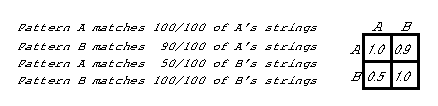
\includegraphics[height=0.6in]{nontex/illustrations/minimalMatrix.eps}
\caption{A similarity matrix created by counting strings matched}
\label{fig:minimalMatrix}
\end{figure}

\begin{figure}[tb]
\centering
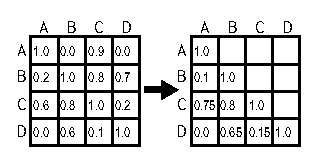
\includegraphics[width=0.7\columnwidth]{nontex/illustrations/matrixToGraph.eps}
\vspace{-6pt}
\caption{Creating a similarity graph from a similarity matrix}
\vspace{-6pt}
\label{fig:matrixToGraph}
\end{figure}



\subsubsection{Overview of process}

The similarity analysis used in this study clusters regular expressions by their behavioral similarity on matched strings.
Consider two unspecified patterns {\tt A} and {\tt B}, a set {\tt mA} of 100 strings that pattern {\tt A} matches, and a set {\tt mB} of 100 strings that pattern {\tt B} matches.
If pattern {\tt B} matches 90 of the 100 strings in the set {\tt mA}, then {\tt B} is 90\% similar to {\tt A}.
If pattern {\tt A} only matches 50 of the strings in {\tt mB}, then {\tt A} is 50\% similar to {\tt B}.
We use similarity scores to create a similarity matrix as shown in Figure~\ref{fig:minimalMatrix}.
In row {\tt A}, column {\tt B} we see that {\tt B} is 90\% similar to {\tt A}.
In row {\tt B}, column {\tt A}, we see that {\tt A} is 50\% similar to {\tt B}.  Each pattern is always 100\% similar to itself, by definition.

Once the similarity matrix is built, the values of cells reflected across the diagonal of the matrix are averaged to create a half-matrix of undirected similarity edges, as illustrated in Figure~\ref{fig:matrixToGraph}.
This facilitates clustering using the  Markov Clustering (MCL) algorithm\footurl{http://micans.org/mcl/}.
We chose MCL  because it offers a fast and tunable way to cluster items by similarity and it is particularly useful when the number of clusters is not known \emph{a priori}.


In the implementation, strings are generated for each pattern using Rex~\cite{rex}.  Rex generates matching strings by representing the regular expression as an automaton, and then passing that automation to a constraint solver that generates members for it\footurl{http://research.microsoft.com/en-us/projects/rex/}.  If the regex matches a finite set of strings smaller than 400, Rex will produce a list of all possible strings.
Our goal is to generate 400 strings for each pattern to balance the runtime of the similarity analysis with the precision of the similarity calculations.

For clustering, we prune the similarity matrix to retain all similarity values greater than or equal to 0.75, setting the rest to zero, and then using MCL.
This threshold was selected based on recommendations in the MCL manual. The impact of lowering the threshold would likely result  in either the same number of more diverse clusters, or a larger number of clusters, but is unlikely to markedly change the largest clusters or their summaries, which are the focus of our analysis for \todoMid{some research question reference}.
, but further study is needed to substantiate this claim.
We also note that MCL can also be tuned using many parameters, including inflation and filtering out all but the top-k edges for each node.
After exploring the quality of the clusters using various tuning parameter combinations, the best clusters (by inspection) were found using an inflation value of 1.8 and k=83.   The top 100 clusters are categorized by inspection into six categories of behavior.

The end result is clusters and categories of highly behaviorally similar regular expressions, though we note that this approach has a tendency to over-approximate the similarity of two regexes. We measure similarity based on a finite set of generated strings, but some regexes  match an infinite set (e.g., \verb!ab*c!), so measuring similarity based on the first 400 strings may lead to an artificially high similarity value. To mitigate this threat, we chose a large number of generated strings for each regex, but future work includes exploring other approaches to computing regex similarity.




\section{Similarity matrix creation}

\subsection{Implementation details}

In clustering the regular expressions, we are most interested in observing behavior of regexes found in multiple projects.  Starting with the 13,597 patterns of the corpus, we discarded 10,015 (74\%) patterns that were not found in multiple projects.
Then we excluded an additional 711 (5\%) patterns that contain features not supported by Rex.  We studied the remaining 2,871 (21\%) patterns using our similarity analysis technique. The impact is that 923 projects were excluded from the data set for the similarity analysis. Omitted features are indicated in Table~\ref{table:featureStats} for Rex.

\subsection{Results}


\section{Markov clustering}
\subsection{Background}
\subsection{Tuning parameters}
\subsection{Results}

From 2,871 distinct patterns, MCL clustering identified 186 clusters with 2 or more patterns, and 2,042 clusters of size 1.
 The average size of clusters larger than size one was 4.5.  Each pattern belongs to exactly one cluster.

Three example strings generated by Rex for the first pattern are: `-()', `*'8(5)', `Oe()'.  For the third pattern, Rex generated these three strings: ` ()', `(q)F', `(n)M'.  The pattern: \verb!\(.*\)$! is very similar, but will not match the string `(n)M', and so was placed in a different cluster.

\begin{table}
\begin{center}
\caption{An example cluster containing 12 regexes, with at least one regex present in 31 different projects.  In this cluster, every regex requires `:'.}
\label{table:exampleCluster}
\begin{small}
\begin{tabular}
{lcc | lcc}
\toprule \bigstrut
\textbf{Index} & \textbf{Pattern} & \textbf{NProjects} & \textbf{Index} & \textbf{Pattern} & \textbf{NProjects} \\
 \midrule \bigstrut
1 & \begin{minipage}{1.6in}\cverb!\s*([^: ]*)\s*:(.*)!\end{minipage} & 9 & 7 & \begin{minipage}{1.6in}\cverb![:]!\end{minipage} & 6 \\
 \midrule \bigstrut
2 & \begin{minipage}{1.6in}\cverb!:+!\end{minipage} & 8 & 8 & \begin{minipage}{1.6in}\cverb!([^:]+):(.*)!\end{minipage} & 6 \\
 \midrule \bigstrut
3 & \begin{minipage}{1.6in}\cverb!(:)!\end{minipage} & 8 & 9 & \begin{minipage}{1.6in}\cverb!\s*:\s*!\end{minipage} & 4 \\
 \midrule \bigstrut
4 & \begin{minipage}{1.6in}\cverb!(:+)!\end{minipage} & 8 & 10 & \begin{minipage}{1.6in}\cverb!\:!\end{minipage} & 2 \\
 \midrule \bigstrut
5 & \begin{minipage}{1.6in}\cverb!(:)(:*)!\end{minipage} & 8 & 11 & \begin{minipage}{1.6in}\cverb!^([^:]*):[^:]*$!\end{minipage} & 2 \\
 \midrule \bigstrut
6 & \begin{minipage}{1.6in}\cverb!^([^:]*): *(.*)!\end{minipage} & 8 & 12 & \begin{minipage}{1.6in}\cverb!^[^:]*:([^:]*)$!\end{minipage} & 2 \\
\bottomrule
\end{tabular}
\vspace{-6pt}
\end{small}
\end{center}
\vspace{-12pt}
\end{table}


Table~\ref{table:exampleCluster} provides an example of a behavioral cluster containing 12 patterns (four longer patterns omitted for brevity). Patterns from this cluster are present in 31 different projects.  All patterns in this cluster share the literal `:' character. The smallest pattern, \verb!`:+'!,  matches one or more colons.

% \begin{figure}[tb]
% \centering
% 
\includegraphics[width=\columnwidth]{nontex/illustrations/clusterEdgesExample.eps}
% \vspace{-12pt}
% \caption{Example Of Similarity Edges Of One Cluster}
% \vspace{-6pt}
% \label{fig:clusterEdgesExample}
% \end{figure}

Another pattern from this cluster, \verb!([^:]+):(.*)!, requires at least one non-colon character to occur before a colon character.  Our similarity value between these two regexes was below the minimum of 0.75 because Rex generated many strings for `:+' that start with one or more colons.
We observe that the smallest pattern in a cluster provides insight about key characteristic that all the patterns in the cluster have in common.  A shorter pattern will tend to have less extraneous behavior because it is specifying less behavior,
yet, in order for the smallest pattern to be clustered, it had to match most of the strings created by Rex from many other patterns within the cluster, and so we observe that {the smallest pattern is useful as a representative of the cluster}.

For the rest of this paper, a cluster will be represented by one of the shortest patterns it contains, followed by the number of projects any member of the cluster appears in, so the cluster in Table~\ref{table:exampleCluster} will be represented as \verb!`:+'(31)!.  This representation is not an attempt to express all notable behavior of patterns within a cluster, but is a useful and meaningful abbreviation.
Other regexes in the cluster may exhibit more diverse behavior, for example the pattern \verb!`([^: ]+):(.*)'! requires a non-colon character to appear before a colon character.
% The eight most common features are found in over 50\% of the projects.
% Shown in Table~\ref{table:featureStats}, the STR and END features are present in over half of the scanned projects containing utilizations.  In our survey, over half (56\%) of the respondents answered that they use endpoint anchors frequently or very frequently, and none of them claimed to never use them.

% The LZY feature  is present in over 36\% of scanned projects with utilizations, and yet was not supported by two of the four major regex projects we explored, brics and RE2.
% In our developer survey, 11\% (2) of participants use this feature frequently and 6 (33\%) use it occasionally, showing a modest impact on potential users.

% When survey participants were asked if they prefer to always use numbered (BKR) or named (BKRN) back references, 66\% (12) of survey participants said that they always use BKR, and the remaining 33\% (6) said ``it depends."  No participants preferred named capture groups.  BKR is present in 5\% of scanned projects, while BKRN is present in only 1.7\%, which corroborates our findings that numbered  are generally preferred over named capture groups.
% \begin{table*}
\begin{center}
\begin{footnotesize}
\caption{How Frequently do Features Appear in Patterns, Files and Projects?}
\label{table:featureStatsOnly}
\begin{tabular}
{lllcccc  cc}
rank & code & example & \% patterns & nPatterns & nFiles & nProjects & nTokens & maxTokens. \\
\toprule[0.16em]
1 & ADD & \begin{minipage}{0.5in}\begin{verbatim}z+\end{verbatim}\end{minipage} & 44.1 & 6,003 & 9,165 & 1,204 & 11,136 & 30 \\
\midrule
2 & CG & \begin{minipage}{0.5in}\begin{verbatim}(caught)\end{verbatim}\end{minipage} & 52.4 & 7,130 & 9,559 & 1,194 & 12,707 & 17 \\
\midrule
3 & KLE & \begin{minipage}{0.5in}\begin{verbatim}.*\end{verbatim}\end{minipage} & 44.3 & 6,017 & 8,163 & 1,099 & 11,620 & 50 \\
\midrule
4 & CCC & \begin{minipage}{0.5in}\begin{verbatim}[aeiou]\end{verbatim}\end{minipage} & 32.9 & 4,468 & 7,648 & 1,026 & 8,179 & 42 \\
\midrule
5 & ANY & \begin{minipage}{0.5in}\begin{verbatim}.\end{verbatim}\end{minipage} & 34.3 & 4,657 & 6,277 & 1,005 & 7,119 & 60 \\
\midrule
6 & RNG & \begin{minipage}{0.5in}\begin{verbatim}[a-z]\end{verbatim}\end{minipage} & 19.3 & 2,631 & 5,092 & 848 & 8,043 & 50 \\
\midrule
7 & STR & \begin{minipage}{0.5in}\begin{verbatim}^\end{verbatim}\end{minipage} & 26.2 & 3,563 & 5,458 & 846 & 3,661 & 12 \\
\midrule
8 & END & \begin{minipage}{0.5in}\begin{verbatim}$\end{verbatim}\end{minipage} & 23.3 & 3,169 & 5,393 & 827 & 3,276 & 12 \\
\midrule[0.12em]
9 & NCCC & \begin{minipage}{0.5in}\begin{verbatim}[^qwxf]\end{verbatim}\end{minipage} & 14.2 & 1,935 & 3,947 & 776 & 2,718 & 15 \\
\midrule
10 & WSP & \begin{minipage}{0.5in}\begin{verbatim}\s\end{verbatim}\end{minipage} & 20.9 & 2,846 & 4,704 & 762 & 6,128 & 32 \\
\midrule
11 & OR & \begin{minipage}{0.5in}\begin{verbatim}a|b\end{verbatim}\end{minipage} & 15.5 & 2,102 & 3,926 & 708 & 2,606 & 15 \\
\midrule
12 & DEC & \begin{minipage}{0.5in}\begin{verbatim}\d\end{verbatim}\end{minipage} & 16.9 & 2,297 & 4,198 & 692 & 4,868 & 24 \\
\midrule
13 & WRD & \begin{minipage}{0.5in}\begin{verbatim}\w\end{verbatim}\end{minipage} & 10.5 & 1,430 & 2,952 & 650 & 2,037 & 13 \\
\midrule
14 & QST & \begin{minipage}{0.5in}\begin{verbatim}z?\end{verbatim}\end{minipage} & 13.8 & 1,871 & 3,707 & 645 & 3,290 & 35 \\
\midrule
15 & LZY & \begin{minipage}{0.5in}\begin{verbatim}z+?\end{verbatim}\end{minipage} & 9.6 & 1,300 & 2,221 & 605 & 1,761 & 12 \\
\midrule
16 & NCG & \begin{minipage}{0.5in}\begin{verbatim}a(?:b)c\end{verbatim}\end{minipage} & 5.8 & 791 & 1,709 & 404 & 1,453 & 28 \\
\midrule
17 & PNG & \begin{minipage}{0.5in}\begin{verbatim}(?P<name>x)\end{verbatim}\end{minipage} & 6.7 & 915 & 1,475 & 354 & 2,399 & 16 \\
\midrule
18 & SNG & \begin{minipage}{0.5in}\begin{verbatim}z{8}\end{verbatim}\end{minipage} & 4.3 & 581 & 1,267 & 340 & 1,159 & 17 \\
\midrule
19 & NWSP & \begin{minipage}{0.5in}\begin{verbatim}\S\end{verbatim}\end{minipage} & 3.6 & 484 & 776 & 270 & 676 & 10 \\
\midrule
20 & DBB & \begin{minipage}{0.5in}\begin{verbatim}z{3,8}\end{verbatim}\end{minipage} & 2.7 & 367 & 647 & 238 & 573 & 11 \\
\midrule
21 & NLKA & \begin{minipage}{0.5in}\begin{verbatim}a(?!yz)\end{verbatim}\end{minipage} & 1 & 131 & 489 & 183 & 148 & 3 \\
\midrule
22 & WNW & \begin{minipage}{0.5in}\begin{verbatim}\b\end{verbatim}\end{minipage} & 1.8 & 248 & 438 & 166 & 408 & 36 \\
\midrule
23 & NWRD & \begin{minipage}{0.5in}\begin{verbatim}\W\end{verbatim}\end{minipage} & 0.7 & 94 & 305 & 165 & 149 & 6 \\
\midrule
24 & LWB & \begin{minipage}{0.5in}\begin{verbatim}z{15,}\end{verbatim}\end{minipage} & 0.7 & 91 & 281 & 158 & 107 & 3 \\
\midrule
25 & LKA & \begin{minipage}{0.5in}\begin{verbatim}a(?=bc)\end{verbatim}\end{minipage} & 0.8 & 112 & 358 & 158 & 133 & 4 \\
\midrule
26 & OPT & \begin{minipage}{0.5in}\begin{verbatim}(?i)CasE\end{verbatim}\end{minipage} & 1.7 & 231 & 377 & 154 & 238 & 2 \\
\midrule
27 & NLKB & \begin{minipage}{0.5in}\begin{verbatim}(?<!x)yz\end{verbatim}\end{minipage} & 0.7 & 94 & 296 & 137 & 117 & 4 \\
\midrule[0.12em]
28 & LKB & \begin{minipage}{0.5in}\begin{verbatim}(?<=a)bc\end{verbatim}\end{minipage} & 0.6 & 80 & 255 & 120 & 99 & 4 \\
\midrule
29 & ENDZ & \begin{minipage}{0.5in}\begin{verbatim}\Z\end{verbatim}\end{minipage} & 0.7 & 89 & 149 & 90 & 89 & 1 \\
\midrule
30 & BKR & \begin{minipage}{0.5in}\begin{verbatim}\1\end{verbatim}\end{minipage} & 0.4 & 60 & 129 & 84 & 73 & 4 \\
\midrule
31 & NDEC & \begin{minipage}{0.5in}\begin{verbatim}\D\end{verbatim}\end{minipage} & 0.3 & 36 & 92 & 58 & 51 & 6 \\
\midrule
32 & BKRN & \begin{minipage}{0.5in}\begin{verbatim}(P?=name)\end{verbatim}\end{minipage} & 0.1 & 17 & 44 & 28 & 19 & 2 \\
\midrule
33 & VWSP & \begin{minipage}{0.5in}\begin{verbatim}\v\end{verbatim}\end{minipage} & 0.1 & 13 & 16 & 15 & 14 & 2 \\
\midrule
34 & NWNW & \begin{minipage}{0.5in}\begin{verbatim}\B\end{verbatim}\end{minipage} & 0 & 4 & 11 & 11 & 5 & 2 \\
\bottomrule[0.13em]
\end{tabular}
\end{footnotesize}
\end{center}
\end{table*}


\subsection{Categorizing behavioral clusters}
From 2,871 distinct regexes, MCL clustering identified 186 clusters with 2 or more regexes, and 2,042 clusters of size 1.
The average size of clusters larger than size one was 4.5.  Each regex belongs to exactly one cluster.  Five example clusters are available in Appendix~\ref{app:top5CompleteClusters}.

A report was prepared from the output of mcl providing the pattern of each regex in each cluster, the number of projects that the regex appears in, the number of projects containing at least one regex from the cluster (how clusters are ranked), and statistics about what features are most used in that cluster.  The contents of this report for the top 20 clusters is available in appendix \todoMid{link}.


\begin{table}
\begin{center}
\caption{An example cluster containing 12 regexes, with at least one regex present in 31 different projects.  In this cluster, every regex requires `:'.}
\label{table:exampleCluster}
\begin{small}
\begin{tabular}
{lcc | lcc}
\toprule \bigstrut
\textbf{Index} & \textbf{Pattern} & \textbf{NProjects} & \textbf{Index} & \textbf{Pattern} & \textbf{NProjects} \\
 \midrule \bigstrut
1 & \begin{minipage}{1.6in}\cverb!\s*([^: ]*)\s*:(.*)!\end{minipage} & 9 & 7 & \begin{minipage}{1.6in}\cverb![:]!\end{minipage} & 6 \\
 \midrule \bigstrut
2 & \begin{minipage}{1.6in}\cverb!:+!\end{minipage} & 8 & 8 & \begin{minipage}{1.6in}\cverb!([^:]+):(.*)!\end{minipage} & 6 \\
 \midrule \bigstrut
3 & \begin{minipage}{1.6in}\cverb!(:)!\end{minipage} & 8 & 9 & \begin{minipage}{1.6in}\cverb!\s*:\s*!\end{minipage} & 4 \\
 \midrule \bigstrut
4 & \begin{minipage}{1.6in}\cverb!(:+)!\end{minipage} & 8 & 10 & \begin{minipage}{1.6in}\cverb!\:!\end{minipage} & 2 \\
 \midrule \bigstrut
5 & \begin{minipage}{1.6in}\cverb!(:)(:*)!\end{minipage} & 8 & 11 & \begin{minipage}{1.6in}\cverb!^([^:]*):[^:]*$!\end{minipage} & 2 \\
 \midrule \bigstrut
6 & \begin{minipage}{1.6in}\cverb!^([^:]*): *(.*)!\end{minipage} & 8 & 12 & \begin{minipage}{1.6in}\cverb!^[^:]*:([^:]*)$!\end{minipage} & 2 \\
\bottomrule
\end{tabular}
\vspace{-6pt}
\end{small}
\end{center}
\vspace{-12pt}
\end{table}

\subsubsection{Representing a cluster with the shortest regex}
Table~\ref{table:exampleCluster} provides an example of a behavioral cluster containing 12 regexes (four longer regexes omitted for brevity). Patterns from this cluster are present in 31 different projects.  All regexes in this cluster share the literal `:' character. The smallest regex, \verb!`:+'!,  matches one or more colons.

% \begin{figure}[tb]
% \centering
% 
\includegraphics[width=\columnwidth]{nontex/illustrations/clusterEdgesExample.eps}
% \vspace{-12pt}
% \caption{Example Of Similarity Edges Of One Cluster}
% \vspace{-6pt}
% \label{fig:clusterEdgesExample}
% \end{figure}

Another regex from this cluster, \verb!([^:]+):(.*)!, requires at least one non-colon character to occur before a colon character.  The behavioral similarity score between these two regexes was below the minimum of 0.75 because Rex generated many strings for `:+' that start with one or more colons.

The smallest regex in a cluster provides insight about key characteristic that all the regexes in the cluster have in common.  A shorter regex will tend to have less extraneous behavior because it is specifying less behavior,
yet, in order for the smallest regex to be clustered, it had to match most of the strings created by Rex from many other regexes within the cluster, and so one minor discovery about clusters of regexes is that {the smallest regex is useful as a representative of the cluster}.

For the rest of this thesis, a cluster will be represented by one of the shortest regexes it contains, followed by the number of projects any member of the cluster appears in, so the cluster in Table~\ref{table:exampleCluster} will be represented as \verb!`:+'(31)!.  This representation is not an attempt to express all notable behavior of regexes within a cluster, but is a useful and meaningful abbreviation.
Other regexes in the cluster may exhibit more diverse behavior, for example the regex \verb!`([^: ]+):(.*)'! requires a non-colon character to appear before a colon character.

% Three example strings generated by Rex for the first regex are: `-()', `*'8(5)', `Oe()'.  For the third regex, Rex generated these three strings: ` ()', `(q)F', `(n)M'.  The regex: \verb!\(.*\)$! is very similar, but will not match the string `(n)M', and so was placed in a different cluster.

% \subsection{Categorization of clusters}
% \subsubsection{Implementation details}
% \subsubsection{Results}


The top 100 largest clusters based on the number of projects were manually sorted into 6 behavioral categories (determined by inspection).  The largest cluster was left out, as it was composed of patterns that trivially matched almost any string, like \verb!`b*'! and \verb!`^'!.  The remaining 99 clusters were all categorized. These clusters are briefly summarized in Table~\ref{tab:clustercats}, showing the name of the category and the number of clusters it represents, patterns in those clusters, and projects. The most common category is \emph{Multi Matches}, which contains clusters that have alternate behaviors (e.g., matching a comma or a semicolon, as in \verb!`,|;'(18)!). Each cluster was mapped to exactly one category.

\begin{table}
\begin{center}
\begin{small}
\caption{Cluster categories and sizes, ordered by number of projects containing at least one pattern in the category. \label{tab:clustercats}}
\begin{tabular}{lcccc}
\toprule
\textbf{Category} & \textbf{Clusters} & \textbf{Patterns} & \textbf{Projects} & \textbf{\% Projects} \\  \midrule \bigstrut
Multi Matches & 21 & 237 & 295 & 40\% \\
\midrule \bigstrut
Specific Char & 17 & 103 & 184 & 25\% \\
\midrule \bigstrut
Anchored Patterns & 20 & 85 & 141 & 19\% \\
\midrule \bigstrut
Two or More Chars & 16 & 40 & 120 & 16\% \\
\midrule \bigstrut
Content of Parens & 10 & 46 & 111 & 15\% \\
\midrule \bigstrut
Code Search & 15 & 27 & 92 & 13\% \\
\bottomrule
\end{tabular}
\vspace{-12pt}
\end{small}
\end{center}
\end{table}


\subsubsection{Six categories of behaviorally similar clusters}
\label{sec:categoriesDefined}
\paragraph{Multiple Matching Alternatives}
The patterns in these clusters match under a variety of conditions by using the CCC or OR feature.  For example: \verb!`(\W)'(89)! matches any alphanumeric character, \verb!`(\s)'(89)! matches any whitespace character, \verb!`\d'(58)! matches any numeric character, and \verb!`,|;'(18)! matches a comma or semicolon.  Most of these clusters are represented by patterns that use default character classes, as opposed to custom character classes.  This provides further support for the survey results to the question, \emph{Do you prefer to use custom character classes or default character classes more often?}, in which a majority of participants indicated they use the default classes more than custom.
This category contains 21 clusters, each appearing in an average of 33 projects.

\paragraph{Specific Character Must Match}
\label{cluster:single}
Each cluster in this category requires one specific character to match, for example:
\verb!`\n\s*'(42)! matches only if a newline is found, \verb!`:+'(31)! matches only if a colon is found, \verb!`%'(22)!, matches only if a percent sign is found and \verb!`}'(14)! matches only if a right curly brace is found.
% Table~\ref{table:exampleCluster} presents a cluster that falls under this category. While the cluster is centered on the presence of the \verb!`:'! character, the other regexes in the cluster also exhibit more diverse behavior.
The commonality of this cluster category contrasts with the survey in
(Section~\ref{sec:surveyResults}) in which participants reported to very rarely or never use regexes to check for a single character (Table~\ref{table:regextasks}).
This category contains 17 clusters, each appearing in an average of 17.1 projects.
These clusters have a combined total of 103 patterns, with at least one pattern present in 184 projects.

\paragraph{Anchored Patterns}
Each of the clusters uses at least one endpoint anchor to require matches to be absolutely positioned, for example:
\verb!`(\w+)$'(35)! captures the word characters at the end of the input, \verb!`^\s'(16)! matches a whitespace at the beginning of the input, and \verb!`^-?\d+$'(17)! requires that the entire input is an (optionally negative) integer.
These anchors are the only way in regexes to guarantee that a character does (or does not) appear at a particular location by specifying what is allowed. As an example, \verb!^[-_A-Za-z0-9]+$! says that from beginning to end, only \verb![-_A-Za-z0-9]! characters are allowed, so it will fail to match if undesirable characters, such as \verb!?!, appear anywhere in the string.
This category contains 20 clusters, each appearing in an average of 15.4 projects.
These clusters have a combined total of 85 patterns, with at least one pattern present in 141 projects.

\paragraph{Content of Brackets and Parenthesis}
\label{cluster:contentparens}
The clusters in this category center around finding a pair of characters that surround content, often also capturing that content. For example,
\verb!`\(.*\)'(29)! matches when content is surrounded by parentheses and \verb!`".*"'(25)! matches  when content is surrounded by double quotes.  The cluster \verb!`<(.+)>'(23)! matches and captures content surrounded by angled brackets.
This category contains 10 clusters, each appearing in an average of 18.4 projects.
 These clusters have a combined total of 46 patterns, with at least one pattern present in 111 projects.
% \todoMid{include this?, and }
\verb!`\[.*\]'(22)!
% \todoMid{matches when content is surrounded by square brackets}

\paragraph{Two or More Characters in Sequence}
\label{cluster:multiple}
These clusters require several characters in a row to match some pattern, for example:
\verb!`\d+\.\d+'(30)! requires one or more digits followed by a period character, followed by one or more digits.  The cluster \verb!`  '(17)! requires two spaces in a row,
\verb!`([A-Z][a-z]+[A-Z][^ ]+)'(11)!,
and \verb!`@[a-z]+'(9)! requires the at symbol followed by two or more lowercase characters, as in a twitter handle.
This category contains 16 clusters, each appearing in an average of 13 projects.
These clusters have a combined total of 40 patterns, with at least one pattern present in 120 projects.

\paragraph{Code Search and Variable Capturing}
\label{cluster:search}
These clusters show a recognizable effort to parse source code or URLs. For example,
\verb!`^https?://'(23)! matches a web address, and \verb!`(.+)=(.+)'(9)! matches an assignment statement, capturing both the variable name and value.
The cluster  \verb!`\$\{([\w\-]+)\}'(11)! matches an evaluated string interpolation and captures the code to evaluate.
This category contains 15 clusters, each appearing in an average of 11.7 projects.
These clusters have a combined total of 27 patterns, with at least one pattern present in 92 projects.


\subsection{Discussion of cluster categories}
When tool designers are considering what features to include, data about usage in practice is valuable.  Behavioral similarity clustering  helps to discern these behaviors by looking beyond the structural details of specific patterns and seeing trends in  matching behavior. Many clusters are defined by the presence of particular tokens, such as the colon for the cluster in Table~\ref{table:exampleCluster}.

\subsubsection{Implications}

\paragraph{Supporting source code parsing.}  One of the six common cluster categories, \emph{Code Search and Variable Capturing}, has a very specific purpose of parsing source code files. This shows a very specific use of regular expressions in practice, occurring in 13\% of all projects containing some clustered regex.  Further study is needed into how users employ regular expressions to parse source code.

\paragraph{Possible bracket parsing bugs.} The \emph{Content of Brackets and Parenthesis} cluster revolves around parsing balanced delimiters, like parenthesis, quotation marks and angle brackets.  Regexes belonging to this category occur in 15\% of all projects containing some clustered regex.  In some cases, parsing balanced delimiters using regexes is known to cause problems for programmers\footurl{http://stackoverflow.com/questions/1732348}, because (most) regular expressions cannot fully describe balanced delimiter rules.  More study is needed into how angle bracket parsing using regex effects source code.

\paragraph{Anchors have a strong behavioral effect.}  Anchors were the only features that had enough of an effect on behavior that clusters formed based on their presence.  Other regexes did not cluster around features, but more instead clustered around characters and character classes.  This implies that certain behaviors can only be specified using anchors.  Of the four regex analysis tools listed in Table~\ref{table:featuresInTools}, only two support the END anchor.  This implies that tool designers should work to better support anchors.

\paragraph{Finding specific content using delimiters.}  Two categorical clusters, \emph{Specific Characters Must Match} and \emph{Two or More Characters in Sequence}, deal with identifying the presence of specific character(s).  While multiple character matching subsumes single character matching, the overarching theme is that these regexes are looking for the presence of very specific content.  More study is needed into what content is most frequently searched for, but this cluster analysis indicates that version numbers, twitter or user handles, hex values, decimal numbers, capitalized words, and particular combinations of whitespace, slashes and other delimiters were discernible targets.

\subsubsection{Threats to validity}
The following threats impact these results and conclusions:

\paragraph{Measures.}  The similarity measure between regexes used in the cluster algorithm is computed empirically rather than analytically, and the more Rex-generated strings used to compute the similarity measure, the more likely it is to be accurate. Our experiments used 400 strings to balance performance and precision, but a higher number could lead to more cohesive clusters. Additionally, regex patters that use any feature not supported by Rex were omitted from the cluster analysis. Last, the threshold of 0.75 was chosen based on the MCL recommendation, but it may not create optimal clusters.

\paragraph{Instrumentation.} Regular expression patterns were clustered using strings generated by the Rex tool. We assume that the strings generated by Rex are reasonably diverse to help characterize the regex behavior. To mitigate this threat, Rex generated 400 strings per regex and we inspected strings randomly to ensure diversity.


